\documentclass[Main]{subfiles}

\begin{document}
%-_-_-_-_-_-_-_-_-_-_-_-_-_-_-_-_-_-_-_-_-_-_-_-_-_-_-_-_-_-_-_-_-_-_-_-_-_-_-_-_-_-_-_-_-_-_-_-_-_-_-_-_-_-_-_-_-_-_-_
%-_-_-_-_-_-_-_-_-_-_-_-_-_-_-_-_-_-_-_-_-_-_-_-_-_-_-_-_-_-_-_-_-_-_-_-_-_-_-_-_-_-_-_-_-_-_-_-_-_-_-_-_-_-_-_
%\newpage
\chapter{Lagrangian Systems and Peierls Brackets}
   %introduzione (Correzione CD)
%  In this chapter we will put to good use all the effort invested in the study of mathematical methods for classical field to provide a good notion of Abstract Mechanical system. 
 % \emph{Abstract} in the sense that we rely on a refined definition, sufficiently broad to encompass mechanical systems with degrees of freedom both discrete and continuous.
 % \\
 % Taking advantage of this language  will be possible to formalize precisely each step of the original Peierls' procedure\cite{Peierls1952} and thus establish the class of applicability of this algorithm.
In this chapter we will take advantage of the language developed in the first chapter in order to  formalize precisely each step of the original Peierls' procedure\cite{Peierls1952} and thus establish the class of applicability of this algorithm. 
  
	\section{Abstract Mechanical Systems}
	%It is possible to state a mathematical definition sufficiently broad to encode all the classical mechanical systems regardless of the cardinality of degrees of freedom  in a unified way. (Correzione CD)
	In what follows we will refer to a rather particular class of dynamical systems:
	
	\begin{definition}[Dynamical System]%Corretto da CD prima era "Evolutive system"
		Pair $(E,P )$ composed of:
		\begin{itemize}
			\item $E \xrightarrow{\pi} M$ \\
			smooth fiber bundle of typical fiber $Q$ on  manifold $M$, called \emph{"configuration bundle"}.
			\item	$ P : \Gamma^\infty(E) \rightarrow \Gamma^\infty(E)$ %\\  operator called \emph{"motion operator"}
		\end{itemize}
	\end{definition}
	This formulation is still very far from the physical interpretation but has the benefit to highlight the minimal mathematical framework
	%to highlight the minimal mathematicalobjects which must be fixed in order to specify a mechanical systems.(correzione CD)
	
	
	\paragraph{Kinematics}
	%Fibrato Configurazione incompassa la cinematica
	The configuration bundle encompasses all the kinematical structures of the system.
	 A pivotal role is played by the smooth sections  which are to be understood as all the possible conformation of the system.

	\begin{definition}[Space of kinematics (off-shell) configurations]
		We call:
		\begin{displaymath}
			\gls{Conf} \coloneqq \Gamma^\infty(M,E)
		\end{displaymath}
		the space of kinematic configurations.
	\end{definition}

	%A section is not a statical configuration, equivalent to a specific point in the configuration space of ordinary classical systems, but has to be seen as a specific realization of the kinematics in the sense of  a complete description of a possible motion. (Correzione CD)
	At this level of abstraction, since no space-time structure has been specified, terms like stasis and motion must be taken with care .The natural physical interpretation should become manifest through the concrete realization of systems with discrete and continuous degree of freedom.
	
	\begin{observation}[Mathematical structure]
	Notice that $\Gamma^\infty(M;E)$ is best understood as an infinite dimensional Manifold. 
	\\
	This framework provides a geometric characterization of the notion of variations as tangent vectors on the the space of kinematic configurations .\cite{Forger2005}
	\end{observation}
	
	\begin{observation}[Coordinate Representation]
	The choice of a chart atlas $\Atlas(M)$ on the base space $M$ and $\Atlas(E)$ on the total space $E$ provides a correspondence between each configuration $\gamma \in \Conf$ and family of smooth real functions $\{f_{\alpha \beta}:A_\alpha \subset \Real^m \rightarrow \Real^q \}$.
	Where $m$ and $q$ are respectively the dimension of $Q$ and $M$.	
	\\
	The process is trivial:
	\begin{displaymath}
		\gamma \in \Conf \mapsto \{f_{A,U}=\psi_U \circ \gamma \circ \psi_A^{-1} \vert (A,\psi_A) \in \Atlas(M), (U,\psi_U)\in \Atlas(E)   \}
	\end{displaymath}
	
	%	$\forall (A,\psi_A)$ local chart on $M$ and $(U,\psi_U)$ local chart on $E$ such that $\gamma(A) \cap U \neq \emptyset$ $f_{A,U}=\psi_U \circ \gamma \circ \psi_A^{-1}$

	Since the whole section is quite difficult to handle  as a global object, is customary in field theory to work in the more practical local representation. 
	\end{observation}	
	
	\begin{observation}[Further specification of the system's kinematics]
	 	The general formalism does not require any other structure to be carried forward.
	 	Additional structure on the fiber , the base or the whole bundle are to be prescribed in order to specify a precise physical model, e.g. the spin structure on $E$ for the Dirac Field.\cite{Benini}
	 \end{observation}	
	
	\paragraph{Dynamics}
	The operator $P$ is the object that contains all the information about the dynamical evolution of the system.
	It has the role to select the dinamically compatible configurations among all the admissible kinematic ones, exactly as it happens in analytical mechanics where the dynamic equations shape the natural motions.
	\begin{definition}[Space of Dynamics (on-shell) configurations]\label{Def:SolSpace}
		We call
		\begin{displaymath}
			\gls{Sol} \coloneqq \ker(P) \subset \Conf
		\end{displaymath}
		the set containing all the smooth solutions of the motion equations corresponding to the  dynamical operator:	
		\begin{displaymath}
			P: \Conf \rightarrow \Conf
		\end{displaymath}
	\end{definition}
	
	\begin{figure}[h!]
		\centering
		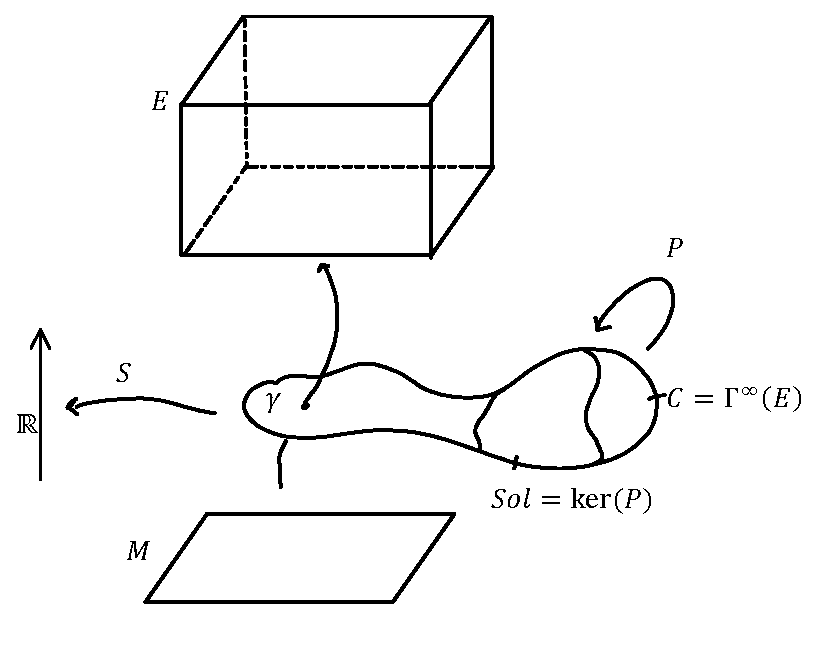
\includegraphics[width=0.5\textwidth]{Pictures/AbstractFieldTheory} 
		 	 	\caption{Mathematimatical framework of the mechanics of abstract systems. }
	\end{figure}	
	
	\subsection{Lagrangian Dynamics}	
	Lagrangian systems constitute an interesting subclass of the abstract dynamical systems:
	%more practical interest:	
		\begin{definition}[Lagrangian System ( of $r$-th order)]
	Pair $(E, \mathcal{L} )$ composed of:
		\begin{itemize}
			\item $E \xrightarrow{\pi} M$ \\smooth fiber bundle of typical fiber $Q$ on the oriented pseudo-Riemmanian manifold $(M,g,\mathfrak{o})$ called \emph{"configuration bundle"}.
			\item	$ \gls{Lagrangian} : J^r E \rightarrow \wedge^m T^*M$ \\bundle-morphism from the r-th Jet Bundle to  the top-dimensionial form bundle over the base manifold $M$  called \emph{"Lagrangian density"} or simply \emph{"Lagrangian"} of r-th order.
		\end{itemize}
	\end{definition}	
	
	\begin{NB}
		In what follows all the systems considered will be exclusively of first order.
		The reason is due to the \emph{Ostrogradsky instability} according to which a non-degenerate Lagrangian dependent on time derivatives of higher than the first corresponds to a linearly unstable dynamics.\cite{Motohashi2014}
	\end{NB}	
	
	
	%la lagrangiana incompassa la dinamica
	In this case, the Lagrangian density is the object containing all the information about the dynamics of the system.

	%In Layman terms la lagrangiana  è un qualcosa che può essere integrato sopra la varietà
	In order to reconstruct the system dynamics from the Lagrangian density has to be understood the mathematical nature of $\Lagrangian$.
	$\Lagrangian$ maps a point $q_p$ on the fiber $J^r_p E$ to a m-form on $T_p M$.
	Recalling the definition of jet bundles it is clear that for each smooth section on $E$ it is associated a smooth section on $J^rE$ :
	\begin{displaymath}
		\phi \in \Gamma^\infty (E) \mapsto (\phi, \partial_\mu \phi, \partial_{\mu, \nu} \phi , \ldots \partial_{\vec{\alpha}}\phi)
	\end{displaymath}
	where  $\vec{\alpha}$ is a multi-index of length r.
	The correspondence is not unambiguous since sections equal up to the r-th order define the same jet section.
	The smoothness of $\Lagrangian$ ensures that each section of the jet bundle is mapped to a smooth section in the top-forms bundle i.e. the most general integrable object on an orientable manifold.
	
	%la classe delle densità lagrangiane
	It should be clear that $\Lagrangian$ is a specific choice among the vast class of functions suitable to be a good Lagrangian density over the  Configuration Bundle $E$:
	\begin{definition}[Lagrangian Density on the bundle $E$]\label{Def:LagrangianDensities}
		\begin{displaymath}
			\gls{Lag}^r (E) \coloneqq \hom\biggr(J^r E,\quad \bigwedge^m( T^*M)\biggr)  \cong \big\{f:\Gamma^\infty(J^r E) \rightarrow \Omega^m(M)  \big\}
		\end{displaymath}
	(where $\Omega^m(M)$ is the common name for $\Gamma^\infty \big( \bigwedge^m( T^*M) \big)$ in the context of Grassmann algebras.)
	The equivalence states the fact that a bundle-morphism induces a map between the sections.
	\end{definition}
	 %this choice fix the "Dynamical identity" of the considered system. (Correzione CD)
	\begin{proposition}
		$\Lag^r(E)$ has an vector space structure inherited by the linear structure of $\Omega(M)$.
	\end{proposition}
	
	
	Thanks to the correspondence between a section $\phi \in \Conf$ and his r-th jet, it is possible to consider the Lagrangian as acting directly on the kinematic configurations.
	%	In layman terms the image  $\Lagrangian [ \phi ] \textrm{d}\mu$ , where $\textrm{d}\mu$ is the measure associated to the orientation $\mathfrak{o}$, is something that can be measured over the whole base space.  (Correzione CD: Non proprio... integrare e misurare sono due cose diverse)
	\\
	This property suggests the introduction of the class of associated functionals:
	\begin{definition}[Lagrangian functional]\label{Def:LagrangianFunctionals}
		We call \emph{Lagrangian functional} a map :
		%Is a functional on $\Conf$ with values on regular distribution over M associated to the generic $\Lagrangian \in \Lag$.	(Correzione CD)
		\begin{displaymath}
			\mathcal{O}_\Lagrangian : \Conf \rightarrow D'(M) \big( C^\infty_0(M) \big)'
		\end{displaymath}			
		where  $D'(M)$ is the space of regular distribution over $M$.
			Such that the Lagrangian functional associated to $\Lagrangian$, valued on the configuration $\phi \in \Conf$ and tested on the test-function $f \in C^\infty_0(M)$ it is given by:
		\begin{displaymath}
			\mathcal{O}_\Lagrangian [\phi] (f) = \int_M \Lagrangian [\phi] f \textrm{d}\mu
		\end{displaymath}		
	\end{definition}	
	
%	\begin{proposition} %(Correzione CD)
%		As a distribution $\mathcal{O}_\Lagrangian [\phi] (f) $ is necessarily linear in the test-functions entry but not in the configurations entry.	
%	\end{proposition}	
	
	\begin{observation}
		The choice of the image of $\mathcal{O}_\Lagrangian$ as a distribution is a necessary precaution to ensure the \emph{convergence} of the functional, whatever is the configuration on which it is evaluated.
		In fact, despite $\Lagrangian [ \phi ]$  being integrable with respect to the measure $\textrm{d}\mu$, it is not necessary summable if the support of the configuration $\phi$ becomes arbitrarily large.
		\\
		This is a simple consequence of the well known sequence of inclusions:
		\begin{displaymath}
			\Lagrangian [ \phi ] \in C^\infty_0(M) \subset L^1_{\textrm{loc}}(M,\mu) \supsetneqq  L^1(M,\mu) 
		\end{displaymath}
		%of the functional analysis . (Correzione CD)
		Indeed, the functional
		\begin{displaymath}
			\mathcal{O}_\Lagrangian [\phi]= \int_{\supp(\phi)} \Lagrangian [\phi] \textrm{d}\mu
		\end{displaymath}
		is well defined for all $\Lagrangian \in \Lag^r(E)$ only over the compactly supported sections. 
		To take account of the global sections it is sufficient to control the integral smearing the integrand with an arbitrary test-function.
	%il funzionale lagrangiana totale e azione
	\end{observation}
	
	\begin{notationfix}
		The functional $\mathcal{O}_\Lagrangian$, when calculated for the specific Lagrangian of the system, takes the name of \emph{Action} or \emph{Total Lagrangian}. 
	\end{notationfix}

	The introduction of the Lagrangian density is meaningless without the prescription of a dynamical principle which allows to determine unambiguously a dynamical operator $P$ on $\Conf$.
	This fundamental principle is the \emph{least action principle}.
	A proper justification of this claim should require the presentation of the differential calculus on the infinite dimensional manifolds $\Conf$. 
	\\
	Jumping straight to the conclusion we can state this correspondence as a law which assigns to all Lagrangian densities an operator on the kinematic configurations space. In the case of a first order Lagrangian we define:
	\begin{definition}[Euler-Lagrange operator]
	We call \emph{Euler-Lagrange operator}, the  differential operator
		\begin{displaymath}
			Q_\chi : \Conf \rightarrow \Conf
		\end{displaymath}
		relative to the Lagrangian density $\chi \in \Lag^1(E)$, such that:
		\begin{equation}
			Q_\chi (\gamma) = \Biggr( \nabla_\mu \biggr( \frac{\partial \chi}{\partial(\partial_\mu \phi)} \biggr\vert_\gamma \biggr) - \frac{\partial \chi}{\partial \phi}\biggr\vert_\gamma \Biggr) \qquad \forall \gamma \in \Conf
		\end{equation}
		Where $\nabla_\mu$ is the covariant derivative corresponding to the background metric $g$.
		($\frac{\partial \chi}{\partial(\partial_\mu \phi)}$ has the be intended as the Lagrangian density constructed differentiating $\chi(\phi, \partial_\mu)$ as an ordinary function, treating its functional entries as an usual scalar variable.)
	\end{definition}
	
	\begin{observation}
		The whole theory of both Lagrangian densities class and Euler-Lagrange equation could be stated in a more syntetic way in terms of a Grassmann-graded variational bicomplex.\cite{Giachetta2009}\cite{Sardanashvily}
	\end{observation}
	
		

%-_-_-_-_-_-_-_-_-_-_-_-_-_-_-_-_-_-_-_-_-_-_-_-_-_-_-_-_-_-_-_-_-_-_-_-_-_-_-_-_-_-_-_-_-_-_-_-_-_-_-_-_-_-_-_-_-_-_-_
%-_-_-_-_-_-_-_-_-_-_-_-_-_-_-_-_-_-_-_-_-_-_-_-_-_-_-_-_-_-_-_-_-_-_-_-_-_-_-_-_-_-_-_-_-_-_-_-_-_-_-_-_-_-_-_
%\newpage
	\section{Concrete Realization}
		In the previous section we stated an abstract definition of Lagrangian systems sufficiently broad to encompass all  classical Lagrangian systems with both discrete degrees of freedom, like particles, and continuous degree of freedom, like fluids or fields.
	Let us show two of the most significant examples.
	%esibiamo quanto è ampia la nostra definizione
	
	
	
		\subsection{Classical Field Theory}\label{Section:CFT}
		%Basically 
		A (classical) \emph{Field System} is nothing more than an abstract Field System $(E,P)$ where the base space $M$  is a suitable spacetime manifold\cite{Bar}. At this stage the question about the Lagrangian nature of the dynamics is purely ancillary.
		\\		
		The idea of taking bundles on a space-time manifold is physically intuitive, kinematically speaking a field configuration is simply the association of some element of the fiber $Q $ for each point of the space-time $M$.
		
		There are, however, a few additional requirements that are often prescribed.
		%prescribed in commonly studied field theories. (correzione CD)
		\paragraph{Linear System Condition}		
			\begin{itemize}
				 \item The configuration bundle $E\xrightarrow{\pi} M$ is a \underline{vector bundle}.
				 \item The motion operator $P$ is a \emph{L.P.D.O.}.
			\end{itemize}
			%Even if it might make sense to speak of nonlinear fields in some more general context, (Correzione CD)
			This condition is a necessary element in case some form of the \emph{superposition principles} as to be taken in account. 
			Obviously this hypothesis is not sufficient to formulate the principle in the strong classical way, i.e.:"the response at a given place and time caused by two or more stimuli is the sum of the responses which would have been caused by each stimulus individually" mostly because only free systems can be considered at this stage and any statement about stimulus can make sense.
			\\
			The first condition, however, ensueres that $\Conf$ is a vector space, in other words every linear combination of kinematic configurations is still a kinematic configuration.
			This condition, together with the linearity of operator $P$,  guarantees that also $\Sol= \ker(P)$ is a linear subspace.		
			 
		\paragraph{Wave-like %Propagative 
			Dynamics Condition}
		\begin{itemize}
			 \item The base manifold $M$ is a \underline{Globally Hyperbolic Spacetime}.
			 \item The motion operator $P$ is \underline{PDE-hyperbolic}\footnote{Hence it is implied that the configuration bundle is linear.}.
		\end{itemize}
		The first condition ensures the existence of Cauchy surfaces and therefore permits to state  \emph{Cauchy Problems} assigning an initial data on such submanifolds.
		Furthermore, PDE-hyperbolicity of the motion operator $P$ guarantees that for every Cauchy surface $\Sigma \subset M$ the corresponding initial data problem is well posed, that is:
			\begin{equation}\label{CauchyProblem}
				\begin{cases} P u = 0 \\ u = u_0 \\ \nabla_{\vec{n}}u= u_1 \\  \vdots \\ \big[\nabla_{\vec{n}} \big]^{k-1}u = u_{k-1}\end{cases}
			\end{equation}
			where $k$ is the order of the linear differential operator as defined in Def. \ref{Def:LPDO},
			admits a unique solution $u\in \Gamma(E)$ for all 
			\begin{displaymath}
				(u_0,\ldots, u_{k-1}) \in \underbrace{\Gamma (\Sigma )\times \ldots \times \Gamma (\Sigma )}_{\footnotesize{ k \textrm{ times}}}
			\end{displaymath}.
			\\
			This suggests the following definition:
			\begin{definition}[Initial Data Set]
				Let be  $P$ a l.d.p.o of order $k$, we call $\gls{Data}$ the set of all the smooth initial data which can be given on the Cauchy Surface $\Sigma$ is:
				\begin{displaymath}
					\Data(\Sigma)  \coloneqq \biggr \{ (f_0,\ldots f_{k-1}) \big \vert f_i \in \Gamma^\infty(\Sigma)\biggr\}  \equiv
					\underbrace{\Gamma^\infty (\Sigma )\times \ldots \times \Gamma^\infty (\Sigma )}_{\footnotesize{ k \textrm{ times}}}					
				\end{displaymath}
			\end{definition}
			\begin{observation}
				$\Data(\Sigma)$ inherit the linear structure of its component $ \Gamma^\infty(\Sigma)$.
			\end{observation}	
			In this term the well-posedness of the Cauchy problem can be stated as follow:

			\begin{proposition}
				The map $$ 	 \gls{SolMap} : \Data (\Sigma ) \rightarrow \Sol $$ which assigns to $(u_0, \ldots, u_{k-1})\in \Data(\Sigma)$ the unique solution of the Cauchy problem \ref{CauchyProblem} is linear and bijective.
			\end{proposition}
			
			Since any solution, when restricted to a generic Cauchy surface $\Sigma'$, determines another n-tuple of initial data, i.e.:
			\begin{displaymath}
				\phi \equiv \SolMap \big(\phi \vert_{\Sigma'}, \nabla_{\vec{n'}}\phi\vert_{\Sigma'}, \ldots, 
				\big[\nabla_{\vec{n'}}\big]^{(k-1)}\phi \vert_{\Sigma'} \big)	\quad \forall \phi\in \Sol
			\end{displaymath}						
			we can define the set of initial data regardless of the particular Cauchy surface:			

			\begin{NB}
			
				Embracing the principle of Ostrogradsky, can be neglected operators of order	beyond the second.
				Without loss of generality we denote the element of $\Data$ as a pair $(f_0,f_1)$.
			\end{NB}			
			
			\begin{definition}[Set of smooth initial Data]\label{Def:DataSenzaSup}
				\begin{displaymath}
					\Data  \coloneqq \frac{\bigsqcup\limits_{\Sigma \in \CauchyClass(M)}\Data(\Sigma)}{\sim} 
				\end{displaymath}
				where $\sim$ is such that:
				\begin{displaymath}
					(f_0, f_1)|_\Sigma \sim (g_0, g_1)|_{\Sigma'} \; \Leftrightarrow \; \SolMap(f_0,f_1) =  \SolMap(g_0,g_1) 
				\end{displaymath}
				\footnotesize{ Initial data, associated with different surface, are equivalent if they lead to the same solution.}	
			\end{definition}
			
			\begin{proposition}
				$\Data$ is a vector space.
			\end{proposition}
			\begin{proof}
				it is sufficient to show that:
				\begin{displaymath}
					\big[ \phi_a + \phi_b \big] = \big[ \phi_a \big] + \big[ \phi_b \big]
				\end{displaymath}
				where $[\phi]= \big\{(\phi\vert_\Sigma , \nabla_{\vec{n}}\phi \vert_\Sigma) \big\vert \Sigma \in \CauchyClass \big\}$.
				In fact:
				\begin{align*}
					 \SolMap_{\Sigma'}\big([(a',b')] + [(c',d')] \big)=\SolMap_\Sigma\big([(a,b)] + [(c,d)] \big) = \SolMap_\Sigma\big([(a,b)] \big)+ \SolMap_\Sigma\big([(c,d)] \big) =\\
					 =\SolMap_{\Sigma'}\big([(a',b')] \big)+ \SolMap_{\Sigma'}\big([(c',d')] \big) = \SolMap_{\Sigma'}\big([(a',b')] +[(c',d')] \big)
				\end{align*}

			\end{proof}
			\begin{corollary}
				The function  $ 	 \SolMap : \Data (\Sigma ) \rightarrow \Sol $ which maps every equivalence class to the associated solution is linear and bijective.
			\end{corollary}
		\begin{observation}
			The hyperbolicity condition  is the main ingredient in the \emph{initial data quantization} procedure\cite{Wald1994}.	
		\end{observation}	
			
		\paragraph{Green-Hyperbolic Dynamic Condition}
		\begin{itemize}
			\item The dynamic is generated by a \underline{Lagrangian}, i.e.  $P= Q_\Lagrangian$.
			\item The motion operator $P$ is a \underline{Green Hyperbolic} L.P.D.O.
		\end{itemize}
		%it is customary in Algebraic quantum field theory to identify quantizable systems through this condition.
		%In fact this condition is a necessary hypothesis to carry on the Peierls construction and the brackets underlie to the definition of the classical symplectic structure.\\ (Correzione CD
		We remark that Green-hyperbolic operators are not necessarily hyperbolic in any PDE-sense, therefore the last two conditions are not equivalent.
		\begin{observation}
			The Green-hyperbolicity condition is a necessary hypothesis to carry on the Peierls construction of the brackets underlying to the definition of the classical symplectic structure.
		\end{observation}	
			 
		\begin{example}
		One can formulate a \emph{Real Scalar Field on curved backgrounds} whitin this abstract picture:
			\begin{center}\begin{tabular}{|l|c|}
			\hline
			Configuration bundle & real scalar field: $F \equiv \Real$\\
													& curved background: $M$ is globally hyperbolic\\
			\hline
			Kinematic Configurations & $\Conf = C^\infty(M,\Real)$\\
			\hline
			Motion Operator			&  $P=\square_M + m^2 + \xi R$ \\
													& normally hyperbolic operator\\
			\hline
			\end{tabular}\end{center}
			Where $P$ is the Klein-Gordon Operator: $\xi$ and $m^2$ are two real numbers, $R$ stands for the scalar curvature build out of $g$ and $\square_M \coloneqq g^ab \nabla_a \nabla_b$ is the d'Alambert operator associated to the Levi-Civita connection.	
			
		Note that this system satisfies all the above three condition.
		\end{example}
	



		\subsection{Finite Degree systems as a Field}\label{MechanicsAsAField}
			With a little more effort it is possible to realize every ordinary mechanic system  -with discrete degrees of freedom- as a special case of classical field.
			
			Consider a Lagrangian system $(Q, L)$ with configuration space $Q$ and Lagrangian function $L: TQ\rightarrow \Real$.
			\\
			Remembering the intuitive meaning of $Q$ as the set of all the statical conformation of the system, it is natural to read as kinematic configuration all and only the trajectories compatible with the constraints.
			In other words the space of kinematic configurations is the set of all the parametrized smooth curves on $Q$:
			\begin{displaymath}
				\Conf = C^\infty(\Real,Q)
			\end{displaymath}
			Therefore, the configuration bundle of this system is the trivial smooth bundle:
			\begin{displaymath}
				E= ( \Real\times Q, \pi, \Real)
			\end{displaymath}
			of typical fiber $Q$, since the corresponding space of sections coincides to  the required configuration space:
			\begin{displaymath}
				\Gamma^\infty(E) \equiv C^\infty(\Real,Q)
			\end{displaymath}

			Also the "field theoretic" picture of the dynamics is not difficult to achieve.
			It is enough to recall how the Euler-Lagrange equation of an ordinary mechanical system can be derived from the \emph{least action principle}:
			\begin{quotation}
				\textbf{Least Action Principle:}
				The %natural (Correzione CD)
				 motions of the mechanical system $(Q,L)$ are the stationary points of the action functional:
				\begin{displaymath}
					S [\gamma]= \int_\Real L(t,\gamma^i, \dot{\gamma}^i) dt
				\end{displaymath}
				constructed from the Lagrangian of the system.
			\end{quotation}
			Remembering that we have interpreted the space $\Real$ of the parameter $t$ as the base manifold of the configuration bundle $E$, it is immediate to see $S$ as the \emph{Total Lagrangian} related to the Lagrangian density:
			\begin{displaymath}
				\Lagrangian[\gamma] \coloneqq L \circ \big( \gamma \big)^{\big\uparrow} dt
			\end{displaymath}
			obtained evaluating the ordinary Lagrangian on the lifted curve $\gamma^\uparrow$ (lift of $\gamma\in \Conf$ from $Q$ to $TQ$).
		
		Summing up, the mathematical structure of such mechanical system is enconded as follows:
			\begin{center}\begin{tabular}{|l|c|}
			\hline
			Configuration bundle & Trivial bundle  $E= Q \times \Real$\\
													& Base manifold: $M=\Real$\\
			\hline
			Kinematic Configurations &  $\Conf=C^\infty(\Real,Q)$\\
			\hline
			Lagrangian Density		&	$\Lagrangian  [\gamma] \coloneqq \big( L \circ	\gamma^\uparrow \big) dt  = L(t,\gamma^i,\dot{\gamma}^i) dt$\\
			\hline
			Motion Operator			&  $P=Q_\Lagrangian \equiv \frac{d}{dt}\big(\frac{\partial}{\partial \dot{x}^i}L\big)-\frac{\partial}{\partial x^i}L $\\
													& normally hyperbolic operator (\danger ?)\\
			\hline
			\end{tabular}\end{center}
			
			Considering that the space $M$ is trivially globally hyperbolic, since every point $t\in\Real$ is a genuine "Cauchy Surface", it is evident how this system can be seen as a special case of field theory: a "field of curves".
			\begin{observation}
				Unless the configuration space is a vector space, the corresponding field theory cannot be linear.
			\end{observation}		
		
%-_-_-_-_-_-_-_-_-_-_-_-_-_-_-_-_-_-_-_-_-_-_-_-_-_-_-_-_-_-_-_-_-_-_-_-_-_-_-_-_-_-_-_-_-_-_-_-_-_-_-_-_-_-_-_
%\newpage
	\section{Hamiltonian Mechanics of Finite Degree systems}
		The picture of the systems with discrete degrees of freedom as a field brings out only a part of the typical mathematical ingredients proper of the \emph{Geometric} approach to the classical mechanics

		\begin{figure}[h!]
		\centering
		\begin{minipage}{0.45\textwidth}
			\centering
			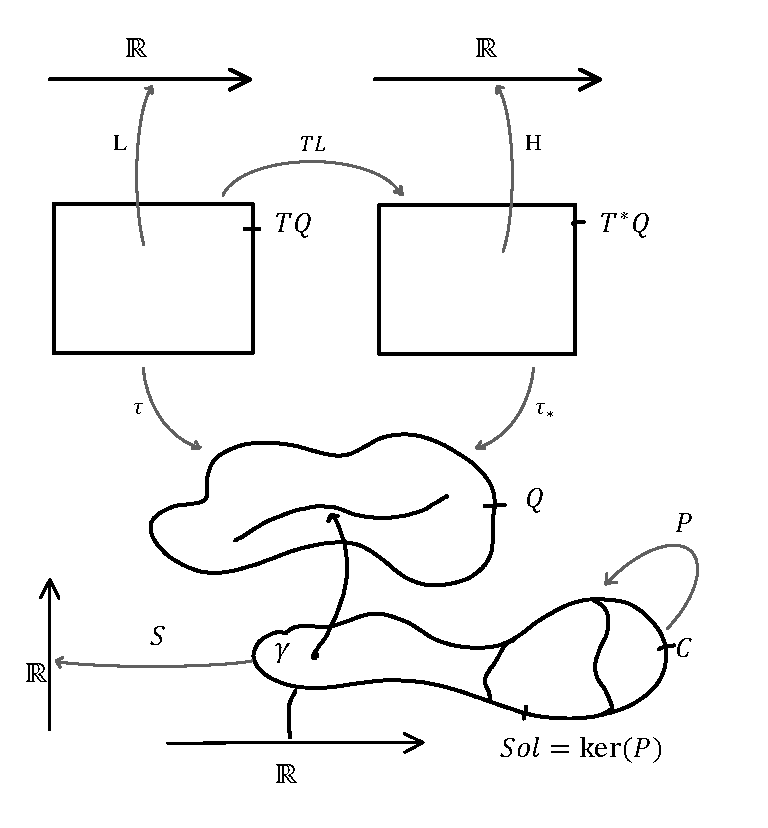
\includegraphics[width=\textwidth]{Pictures/GeoMecFrame} 
			%\caption{first figure}
		\end{minipage}\hfill
		\begin{minipage}{0.45\textwidth}
			\centering
			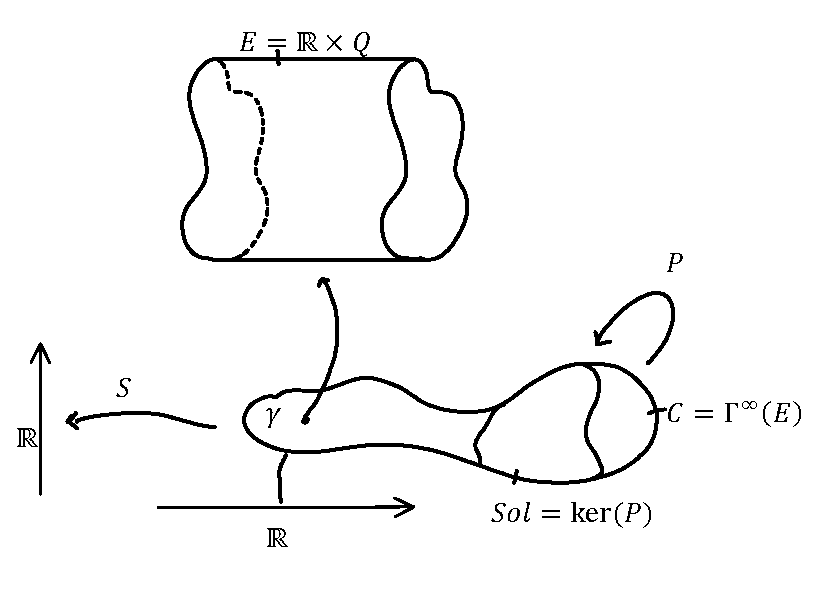
\includegraphics[width=\textwidth]{Pictures/FieMecFrame} 
			%\caption{second figure}
		\end{minipage}
		\caption{An "impressionistic comparison"  between the mathematical framework of geometrical mechanics and  the field-theoretic picture}
		\end{figure}
	
	For example we have a ovvoided to mention the Hamiltonian formalism in the case of abstract fields.
	Even though it should be possible, in the spirit of what has been done within the Lagrangian picture, to extend the canonical treatment to include systems with continuous degrees of freedom (see for example \cite{Giachetta1999}),we will not expand this topic since the protagonist of this thesis is essentially a classical point particle system.
	
	%However in the next chapter we will need to realize a field-theoretic versions of some Canonical objects.	\\  (Correzione CD)
	To fulfill these quantization procedures we will need to draw inspiration from their correspondent classical versions.	Let us briefly review them in the finite dimensional case,
	
			\paragraph{Phase Space}
		We recalled in chapter 1 the definition of \emph{Phase Space} in ordinary classical mechanics as the cotangent bundle $T^*Q$ of the classical configuration space $Q$.
		We showed that every classical phase space is symplectic trough the natural Poincaré form.
		Nevertheless  every quantization procedure requires a modification of this standard symplectic form in order to implement the canonical commutation relations.
	
	This leads us to make use of the abstract formulation of Hamiltonian systems\cite{Abraham1978}:
	
	\begin{definition}[(Ordinary) Hamiltonian System]
			Triple $(\Phase,\omega, H )$ composed of:
		\begin{itemize}
			\item $(\Phase,\omega)$ \\ finite dimensional symplectic manifold called \emph{"Phase space"}.
			\item	$ H :\Phase \rightarrow \Real$ \\  smooth function called \emph{"Hamiltonian"}
		\end{itemize}
	\end{definition}
	
	\begin{observation}
		In classical mechanics Hamiltonian systems could be seen as a subset of Lagrangian systems.
		\\
		The key is the definition of the Legendre Map $TL: TQ \rightarrow T^*Q$,  in the case that the Lagrangian $L$  is \emph{hyperegular}  - i.e. $TL$ is a diffeomorphism - is possible to push-forward $L$ to give a proper Hamiltonian on $\Phase=T^*Q$. (see for example \cite{Abraham1978})
	\end{observation}	
	Recall that the Darboux theorem states that, at least locally, every symplectic form can be represented in the canonical form:
	\begin{theorem}[Darboux]
		$ $
		\begin{hypothesis}
			\begin{itemize}
				\item $\Phase$ is a 2n-dimensional smooth manifold.
				\item $\omega$ is a symplectic form on $\Phase$ i.e. a non degenerate closed ($d \omega =0$) two-form.
			\end{itemize}
		\end{hypothesis}
		\begin{thesis}
			 $\forall m\in \Phase$,  $\exists$ a local chart  $(U,\varphi)$ (where $\varphi(u) = \big(x^1(u), \ldots, x^n(u); y^1(u),\ldots, y^n(u) \big)$) such that:
					\begin{itemize}
						\item $\varphi(m) =0$
						\item	$\omega \big\vert_U = \sum_{i=1}^n dx^i \wedge dy^i$
					\end{itemize}
		\end{thesis}
	\end{theorem}
	\begin{proof}
		We omit the proof which can be found in \cite{Abraham1978}[Th. 3.2.2].
	\end{proof}		
		
	\paragraph{Classical Observables}
		Observables in classical mechanics are represented by real valued smooth functions on $\Phase$:
	\begin{notationfix}
		The \emph{Space of Classical Observables} is denoted as:
		\begin{displaymath}
			\Obs \equiv		C^\infty(\Phase,\Real)
		\end{displaymath}
	\end{notationfix}
	\begin{observation}
		The space  $C^\infty(\Phase,\Real)$ of smooth real valued function on $\Phase$,  inherits the structure of commutive algebra over $\Real$ from its codomain $\Real$.
	\end{observation}
	The symplectic structure on $\Phase$ gives rise to a second algebraic structure on the vector space of observables.
	At first it is necessary to introduce the Hamiltonian fields:
	\begin{definition}[Hamiltonian field with energy function $H\in \Obs$]
		Is the vector field $\mathbf{X}_H$ determined by the condition:
		\begin{displaymath}
			\omega( \mathbf{X}_H,  \cdot )\equiv dH (\cdot)
		\end{displaymath}
	\end{definition}
	Nondegeneracy of $\omega$ guarantees that $\mathbf{X}_H$ exists for all classical observables $H\in \Obs$.
	From that follows the definition of the bracket:
	\begin{definition}[Poisson Brackets]
		Is the bilinear function 	$\{\cdot, \cdot\} : \Obs \times \Obs \rightarrow \Obs$ such that:
		\begin{equation}
			\{ f, g \} \coloneqq \omega \big( \mathbf{X}_f , \mathbf{X}_g \big) = df ( \mathbf{X}_g)
		\end{equation}
	\end{definition}	
	
	In the canonical coordinates, provided  by  Darboux theorem, the  Poisson bracket assumes the typical expression:
	\begin{proposition}[Symplectic coordinate representation]
	
	In canonical coordinates  $(q^1, \ldots, q^; p_1, \ldots, p_n)$ we have:
	\begin{equation}\label{Eq:SymplecticCoordinateRepresentation}
		\{f,g\} = \sum_{i=1}^n \biggr(\frac{\partial f}{\partial q^i} \frac{\partial g}{\partial p_i}  - \frac{\partial f}{\partial p_i} \frac{\partial g}{\partial q^i} \biggr) \qquad \forall f,g \in \Obs
	\end{equation}
	\end{proposition}
	\begin{proof}
			We omit the proof which can be found in \cite{Abraham1978}[Corol. 3.3.14].
	\end{proof}

	\paragraph{Solution Space}
	In this framework the Hamilton's equations of motions can be written in terms of the Hamiltonian Fields:
				\begin{quotation}
				\textbf{Hamilton dynamics principle}
				The dynamically allowed configurations for $(\Phase,H)$ corresponds to the \emph{ integral curves}\cite{Abraham1978} of the Hamiltonian vector field $X_H \in \Gamma(T\Phase)$
			\end{quotation}
		It follows that the specification of a point in the phase space is an appropriate initial data for determining a solution of Hamilton's equations of motion, \textit{i.e}, each point $y\in \Phase$  gives rise to a unique solution of the dynamical evolution.
		Therefore:
		\begin{equation}\label{Eq:PhaseDataSol}
			\Phase \cong \Data \cong \Sol
		\end{equation}
	
	\subsection{Linear dynamical systems}\label{Section:LinearClassicalSystem}
	Most of the physical systems that are encountered in the theory of fields are linear.	
	It is possible to come across linear dynamical systems also in ordinary mechanics. 
		\begin{remark}
			\textbf{Linear Hamiltonian System}
			\begin{itemize}
				\item $\Phase$ has a natural structure of vector space.
				\item	$H$ is a quadratic function on $\Phase$.\footnote{Equations of motion are then linear on the affine canonical coordinates. Dynamics is thus simply a collection of coupled harmonic oscillators.}
			\end{itemize}
		\end{remark}

	In this case the the difference between the underlying geometric entities tends to fade out as a consequence of the flatness of the configuration space.
	
	The key consequence of the vector structure of $\Phase$  is that it allows us to identify the tangent space at any point $y \in \Phase$ with the Phase space $\Phase$ itself.
	Under this identification, the symplectic form becomes a bilinear function $\Omega: \Phase \times \Phase \rightarrow \Real$ on $\Phase$, \textit{i.e.}, It can be seen as acting directly on the points of the phase space rather than on tangent vectors.
	In this way, the phase space of a linear dynamical system, may be viewed  as a \emph{symplectic vector space} $(\Phase, \Omega)$.
	
	Due to the identification of the phase space and the solution space, follow that the symplectic structure $\Omega$ is directly transferred from $\Phase$ to $\Sol$. This symplectic vector space structure $( \Sol	, \Omega)$ of the manifold of solutions for a linear dynamical system is the fundamental classical structure that underlies the construction of the \emph{Inital Data} quantization procedure.
	
	In light of the linear structure the \emph{Linear Observables} take a primary role:
	\begin{displaymath}
		\Obs_{\textrm{lin}} = \Phase^*
	\end{displaymath}
	This set is a vector space and every choice of linear canonical coordinates $\psi^\alpha = (q^a, p^b)$ on $\Phase$ constitutes a  basis on $\Obs_{\textrm{lin}} $:
	\begin{displaymath}
		T\Phase \simeq \Phase \; \Rightarrow \; d\psi^\alpha \equiv \psi^\alpha
	\end{displaymath}
	$\Phase_{\textrm{lin}}$ forms a Poisson subalgebra.
	\\%Moreover, 
	The presence of the non-degenerate bilinear form provide the usual identification $\Phase \simeq \Phase^*$ and therefore the simplectic form on $\Phase$ can directly reproduced on $\Obs{\textrm{lin}} $:
	\begin{displaymath}
		\{ \Omega(y_1, \cdot),\Omega(y_2, \cdot)\} = - \Omega(y_1, y_2) \qquad \forall y_i \in \Phase \Rightarrow \Omega(y_1, \cdot) \in \Obs_\textrm{lin}
	\end{displaymath}

	
	
	
	\begin{TAM}
			To summarize the essential aspects that characterize the geometry of linear systems are the following:
		\begin{itemize}
			\item The symplectic form of $\Phase$ is directly defined on the points of the Phase space.
			\item Since the points of the phase space can be put in correspondence with the solutions (can be considered as the \emph{inital data} ) the symplectic form is directly transported to $\Sol$.
			\item The same simplectic structure can be reproduced on the space $\Obs_\textrm{lin}$ and coincides with the reduction of the Poisson bracket to this subspace.
			\end{itemize}
	\end{TAM}


%-_-_-_-_-_-_-_-_-_-_-_-_-_-_-_-_-_-_-_-_-_-_-_-_-_-_-_-_-_-_-_-_-_-_-_-_-_-_-_-_-_-_-_-_-_-_-_-_-_-_-_-_-_-_-_-_-_-_-_
%-_-_-_-_-_-_-_-_-_-_-_-_-_-_-_-_-_-_-_-_-_-_-_-_-_-_-_-_-_-_-_-_-_-_-_-_-_-_-_-_-_-_-_-_-_-_-_-_-_-_-_-_-_-_-_
%\newpage
	\section{Peierls Brackets}
		Purpose of the Peierls' procedure is to provide a bilinear form on the space of Lagrangian densities with time-compact support.
		This form induces a pre-symplectic structure on suitable subspaces of functionals to which can be recognized the role of \emph{classical observables}  of the theory.	
	
	\begin{observation}[Relation between Peierls Brackets and Poisson Brackets]
		Intuitively we can say that the Peierls Brackets implement a sorts of "comparison relation" between two observables similar to the Poisson brackets in ordinary Hamiltonian mechanics.
		
		As we will see there are important differences between the two definitions:
		\begin{itemize}
			\item The Poisson brackets determines how one "quantity" $b$ changes another "quantity" $a$ when it acts as the  generator (tipically the  Hamiltonian) of the dynamical evolution or vice-versa. \cite{Sharan2010}
	\\	
	The Peierls brackets, on the other hand, determines how one "quantity" $b$  when added to the system dynamics (usually the Lagrangian or the total action)  with an infinitesimal coupling constant $\lambda$ affects changes in another "quantity" $a$ and vice-versa.
	
	%In other words the Peierls brackets are related to the change in an observable when the trajectory on which it is evaluated gets shifted due to an infinitesimal change in the Lagrangian of the system by a second Lagrangian density.
	In other words the Peierls brackets are related to the change in an observable when the trajectory on which it is evaluated gets shifted.
	The shift is not arbitrary, is determined by an infinitesimal change in the Lagrangian of the system through the addition of a second Lagrangian density.
	
			\item While the Poisson brackets between two observables $a$ and $b$ is defined on the whole phase space and is not dependent on the existence of a Hamiltonian, the Peierls brackets refers to a specific trajectory determined by a given Lagrangian. 
		\end{itemize}
		A rigorous treatment of the notions of \emph{observable} and \emph{Phase Space} should require some further specification depending on which is the  considered brackets.		
		We can read the "observable" as an object with a twofold nature. Essentialy it can act both as the generator of the dynamics and as a quantity which can be evaluated on the system configurations.
	\end{observation}	
	
	%Intro: riproponiamo in modo esteso la costruzione originale di peierls con alcuni aggiornamenti di marolf... per una carrellata con il linguaggio della moderna teoria dei campi classici (tipo mangiaratti) e in presenza di gauge vedere per esempio Khavkine
		In this section we present more extensively the original Peierls' construction. 
		Please note that we are not trying to provide the state of the art on the Peierls brackets ( see for example \cite{Khavkine2014} for the treatment in presence of gauge freedom) but only to expand and modernize the first approach given by Peierls.
	Instead of considering only a scalar theory we extend the algorithm to a broader class of systems.
	
	\subsection{Peierls' construction.}
			%Classe di applicabilità naturale del metodo di Peierls
	The Peierls's construction algorithm is well defined for a specific class of systems:
		\begin{enumerate}[(A)]
			\item\label{HpPeierls1} Linear field theory: $E=(E,\pi,M)$ is a vector bundle.
			%\item  Lagragian dynamics: $P=Q_\Lagrangian$ is a L.P.D.O.
			\item\label{HpPeierls2} $P=Q_\Lagrangian$ is a Green-hyperbolic linear partial differential operator.
			\item\label{HpPeierls3} $M$ is a globally Hyperbolic space-time.
			%\item Motion operator $P$ is a Green-hyperbolic.
		\end{enumerate}	
	The procedure can be summarized in a few steps:
	\begin{enumerate}
		\item Consider a \emph{disturbance} $\chi$ that is a time-compact Lagrangian density .
		\item Construct the \emph{perturbation of a solution under the action of $\chi$}.
		%\emph{perturbation of a solution under the disturbance}. (correzione CD
		\item Define the \emph{effect of the disturbance} on a second Lagrangian functional.
		\item Assemble the mutual effects of two different Lagrangian densities to give a \emph{brackets}.
	\end{enumerate}	
	Let us review each step in details.
	
	\subsubsection{Disturbance and Disturbed motion operator }
		By \emph{"disturbance"} we mean a time-compact supported Lagrangian density $\chi \in \Lag$\footnote{I.e. the top form $\chi(\phi)$ is time-compact supported for all $\phi \in \Conf$.} which acts as a perturbation on the system's Lagrangian:
		\begin{displaymath}
			\Lagrangian \rightsquigarrow \Lagrangian' = \Lagrangian + \epsilon\cdot \chi
		\end{displaymath}
		where $\epsilon$  is a real modulation parameter.
		The support condition is required in order to take in account only perturbations which affect the dynamic for a definite time interval.
		The ruling operator of the perturbed dynamics is:
		\begin{equation}
			P_\epsilon = \Biggr[ \nabla_\mu \biggr( \frac{\partial \Lagrangian}{\partial(\partial_\mu \phi)} \biggr) - \frac{\partial \Lagrangian}{\partial \phi} \Biggr] + \epsilon \Biggr[ \nabla_\mu \biggr( \frac{\partial \chi}{\partial(\partial_\mu \phi)} \biggr) - \frac{\partial \chi}{\partial \phi} \Biggr]
			= P + \epsilon Q_\chi		
		\end{equation}
		\begin{observation}
			$P_\epsilon$ is not necessary linear, hypothesis \ref{HpPeierls2} guarantees the linearity only for $P$.
		\end{observation}

	\subsubsection{Solution of the disturbed motion}
		The second ingredient of the Peierls' procedure is the calculus of the \emph{perturbed solutions} under the considered \emph{disturbance}.
		\\
		These are obtainable by a infinitesimal linear perturbation of any, but fixed, solution $\phi \in \Sol$. The good definition of linear superposition is guaranteed by the hypothesis \ref{HpPeierls1}.
		 %These are the solutions $\phi'\in \Conf$ of $P_\epsilon$ obtainable by a infinitesimal linear perturbation of a fixed solution $\phi \in \Sol$. The good definition of linear superposition is guaranteed by the hypothesis 1).(Correzione di CD)
		More precisely, one looks for to be seek a configuration:
			\begin{displaymath}
					\phi'(x) = \phi(x) + \epsilon \eta(x) \in \Conf
			\end{displaymath}
		such that:
			\begin{align*} 
				P_\epsilon \phi'(x) &= o(\epsilon)  \\ 
				P \phi(x) &= 0
			\end{align*}
		In other word the following equation has to be satisfied:
		\begin{displaymath}
			\big[P_\epsilon\big] \phi'(x) = \big[ P + \epsilon Q_\chi		\big]( \phi(x) + \epsilon \eta(x)) 
			= \epsilon \biggr( \big[P\big] \eta(x) + \big[Q_\chi \big]( \phi(x) + \epsilon \eta(x)\big)\biggr) \mbeq o(\epsilon)			
			%= \epsilon \big( P \eta(x) + Q_\chi \phi(x) \big)+ \epsilon^2 Q_\chi	\eta(x) \mbeq o(\epsilon)
		\end{displaymath}
		The linearity condition for operator $P$ does not hold true in general for $Q_\chi$.
		We can work around this problem considering the linearization\cite[pag. 31]{Khavkine2014} of $Q_\chi$ around the unperturbed solution $\phi(x)$. 
		The linearization of $Q_\chi$ is the unique linear operator $\big[Q_\chi^{lin}(\phi) \big]$ such that:
		\begin{displaymath}
			\big[Q_\chi \big]( \phi(x) + \epsilon \eta(x)\big)= \big[Q_\chi \big]( \phi(x)) + \epsilon \big[Q_\chi^{lin}(\phi)  \big]( \eta(x)) + o(\epsilon)
		\end{displaymath}
		which can be seen as the first term of a \emph{formal} Taylor expansion of operator $Q_\chi$ around $\phi$\footnote{If $\Conf$ is a Frechet manifold the expansion could be stated rigorously by defining $\big[Q_\chi^{lin}(\phi_0) . \big] = \big[\dfrac{\partial Q_\chi}{\partial \phi} (\phi_0)\big] $ in terms of the Gateux derivative.}
		This is reflected in a condition on the perturbation $\eta \in \Conf_{tc}$:
		\begin{displaymath}
			\big[P_\epsilon\big] \phi'(x) =  \epsilon \biggr( \big[P\big] \eta(x) + \big[Q_\chi \phi(x) \big]\biggr)+ \epsilon^2 \big[Q_\chi^{lin}(\phi)  \big]	\eta(x) \mbeq o(\epsilon)
		\end{displaymath}
		\begin{equation}\label{PeierlJacobiEqLin}
			\Rightarrow P \eta = - Q_\chi \phi(x)
		\end{equation}
		called \emph{Jacobi Equation}.
		This equation is a non homogeneous P.D.E. with inhomogeneous term $ (- Q_\chi \phi(x))$ fixed by the solution $\phi\in \Sol$ to be perturbed.

		It follows from the definition of Green hyperbolicity that the domain restrictions of $P$ to $\Gamma^\infty_{\textrm{pc}}$ or $\Gamma^\infty_{\textrm{fc}}$ admit a unique inverse $G^+$ and $G^-$ respectively.
   		Therefore, equation \ref{PeierlJacobiEqLin} admits a unique past compact solution $\eta_+$, called retarded perturbation of $\phi\in \Sol$, and a unique future compact solution $\eta_-$, called advanced perturbation:
   		\begin{equation}\label{Perturbation}
   			\eta_\pm = G^\pm \big( - Q_\chi \phi \big)
   		\end{equation}
   		Note that the time-compact support condition on $\chi$ guarantees that $Q_\chi \phi \; \in \dom(G^+) \cap \dom(G^-)$.
   		Expression \ref{Perturbation} reflects perfectly the orginal Peierls' notation where $\eta_\pm$ were noted as functions of the unperturbed solution: $\eta_+ \equiv\reflectbox{\reflectbox{D}}_\chi \phi$ and $\eta_- \equiv  \reflectbox{D}_\chi \phi$.
		
		
		\begin{observation}
			In most of the practical cases it is possible to give a more "down to earth" characterization of $\eta_\pm$ in terms of a Cauchy problem.\\
			It has to be stressed that this approach is not possible in general since Green-hyperbolic operators are not necessarily hyperbolic in any PDE-sense i.e. the well-posedness of the Cauchy problem is not guaranteed on any Cauchy surface. \cite[pag 1]{Bar} \cite[remark 3.18]{Bar2010}\cite[remark 2.1]{Khavkine2014}
			\\
		Consider a motion operator $P$ which is also hyperbolic.
		Taking in account the time-compact support condition of $\chi$, is possible to pick up  two Cauchy surfaces $\Sigma_\pm$ ( $+$ is after the perturbation while $-$ stands for prior to the perturbation) such that:
		\begin{displaymath}
			J^\mp (\Sigma_\pm) \supset \supp(\chi) 
		\end{displaymath}
		for all time-slice foliations of the globally hyperbolic space-time.

		For each of these two surfaces a Cauchy problem can be posed:
		\begin{equation}\label{PerturbationCauchyProblem}
		   \begin{cases}
			   P \eta = - Q_\chi \phi \\
			   (\eta, \nabla_n \eta ) \big \vert_{\Sigma_{\pm}} = (0,0)
   			\end{cases}
   		\end{equation}
   		which , according to the well-posedness of the Cauchy problem, admits an unique solution.
   		The link with the previous presentation is that past/future -compact supported configurations trivially meet the initial data condition for some future/past Cauchy surface.
		\end{observation}
		
		In conclusion, for any but fixed $\phi\in \Sol$ and perturbation $\chi$, there exist two uniquely perturbed solutions:
		%In conclusion,fixed a solution $\phi\in \Sol$ and a perturbation $\chi$, are uniquely determined two perturbed solution: (Correzione CD)
   		\begin{equation}\label{PerturbedSolution}
   			\phi^\pm_\epsilon = \phi + \epsilon \eta_\pm
   		\end{equation}
   		such that:
 		\begin{center}   \begin{tabular}{|c|c|c|c|}
   		\hline
  	 		\emph{retarded pertubation} & $\eta_+ \in \Gamma^\infty_{pc}$ & $(\eta_+, \nabla_n \eta_+ ) \big \vert_{\Sigma_{-}} = (0,0)$ & "propagating forward" \\
  	 		\hline
   			\emph{advanced pertubation} &$\eta_- \in \Gamma^\infty_{fc}$ & $(\eta_-, \nabla_n \eta_- ) \big \vert_{\Sigma_{+}} = (0,0)$ & "propagating backward" \\
   			\hline
   		\end{tabular}	\end{center} 	
		
			
   		
		\subsubsection{Effect Operator}
		Considering an arbitrary continuous\footnote{The precise notion of continuity require the specification of a (infinite dimensional) manifold structure on $\Conf$.} functional $B: \Sol \rightarrow \Real$ (not necessarily linear) we can define the effect of a perturbation on the values of $B$\cite[pag. 5]{Marolf1993} as a map:
		\begin{displaymath}
			\gls{EffectOp} : C^1(\Sol,\Real) \rightarrow C^1(\Sol,\Real)
		\end{displaymath}
		\begin{equation}\label{EffectOperator}
		\EffectOp_\chi^\pm B ( \phi_0) 
		\coloneqq \lim_{\epsilon \rightarrow 0}
		 \biggr( \frac{B(\phi_\epsilon^\pm) - B (\phi_0)}{\epsilon} \biggr)
		\end{equation}
		The advanced and retarded effects of $\chi$ on B are then defined by comparing the original system with a new system defined by the same kinematic configuration space $\Conf$ but with perturbed Lagrangian.
		\begin{observation}
			Expression \ref{EffectOperator} is clearly a special case of Gateaux derivative.\cite{Blanchard2015}
		\end{observation}
		
		
		The former expression simplifies in case of a linear functional:
			\begin{equation}\label{EffectOperatorLinear}
				\EffectOp_\chi^\pm B ( \phi_0) =  B(\eta_\pm)
			\end{equation}
		
		\subsubsection{The Brackets}
		Remembering that every Lagrangian density define a continuous functional (Action).
		From that is possible to build a binary function:
		\begin{displaymath}
			\{\cdot,\cdot\}:\Lag_{\textrm{tc}} \times \Lag_{\textrm{tc}} \rightarrow \Real 	
		\end{displaymath}
		as follow:
		\begin{equation}\label{AbstractPeierlsBracket}
				\{\chi, \omega \}(\phi_0) \coloneqq \EffectOp_\chi^- F_\omega (\phi_0) - \EffectOp_\chi^+ F_\omega(\phi_0)
		\end{equation}

		\begin{proposition}[Bilinearity]
			When restricted to Linear Lagrangian densities $\{\cdot,\cdot\}$ is a bilinear form
		\end{proposition}
		\begin{proof}
			Linearity in the first entry follows from equation\ref{Perturbation} and the linearity of the Euler-Lagrange operator $Q_\cdot$ over $\Lag$.
			\\
			Linearity in the second entry is guaranteed only for Lagrangian densities $\omega$ which provide a linear Lagrangian Functional $F_\omega$.
		\end{proof}
		We are not interested in addressing the cases for which the simplectic property is met on this general ground. 
		In the next chapter we will face the problem to determine  symmetry and non-degeneracy properties for the case of  \emph{classical observable functionals}, a subclass of Lagrangian functionals of most practical use in the quantization schemes.

	\subsection{Extension to non-linear theories}\label{Section:NonLinearPeierls}
		In the previous construction the Green-hyperbolicity of $P$ plays a primary role.
		The problem of searching perturbed solution to the disturbed dynamic can be stated even in presence  of non-linear fields  when the configuration bundle is not necessary a vector bundle or the operator ruling the dynamics is not linear.
		\begin{figure}[h!]
				  \centering
			   	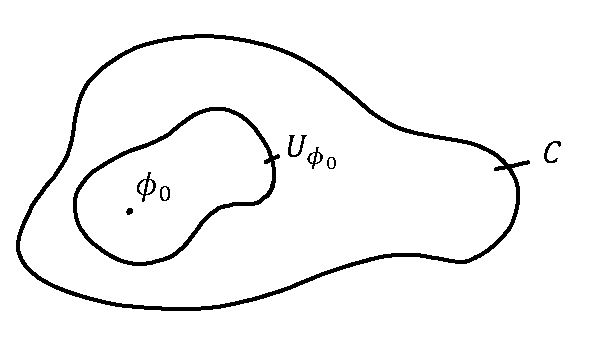
\includegraphics[width=0.5\textwidth]{Pictures/Linearization} 
   	  			\caption{Intrinsically, searching a variation of a solution $\gamma_0\in \Sol$ which solve the disturbed motion equation is equivalent to find the intersection of the perturbed solution with a local neighbourhood of $\Gamma_0$ : $U_{\gamma_0}\cap\ker(P_\epsilon)$ .}
		\end{figure}		
		
		The crucial point of the Peierls' procedure  is to select among all the possible solutions of the perturbed motion $P_\epsilon$ that configuration which can be constructed by a variation of a given solution of the non-perturbed dynamics $\gamma_0 \in \Sol$.
		In this sense the problem results in a \emph{"linearization"} inasmuch the  search of such solution is restricted to a local neighbourhood of the "point" $\gamma_0\in \Sol$.

		Previously the choice to consider only the linear variation was quite natural but in the general case this preferential restriction is no longer possible.
		Anyway, it is possible to  recover a notation similar to \ref{PerturbedSolution} by working patchwise, under the choice of a particular coordinate representation.
		\\
		Fixed a solution $\gamma_0 \in \Sol$ and a local trivializing chart $(A, \phi_A)$ such that $A\cap \ran(\gamma_0) \neq \emptyset$ we can define a local infinitesimal variation by acting on his components:
		\begin{displaymath}
			\gamma_\lambda ^{\, i}(x) = \gamma_0^{\, i}(x) + \lambda \eta^i(x) \qquad \forall x\in \pi(A)
		\end{displaymath}
		where $ \gamma_0^{\, i}$ are the component of the unperturbed solution in the open set $A$ and $\eta^i\in \Real^q$ is a generic real q-ple ( q is the dimension of the typical fiber).
		$\lambda$ is a real parameter that has to be "sufficiently small" in order to guarantee that the range of $\gamma_\lambda$ is properly contained in $A$.
		\\
		In other words the construction of the linear variation, that for linear field theories could be done in a global way, in the general case can be recovered only locally varying the components.
		
		Therefore it is possible to define the effect of a disturbance locally, searching a local section $\gamma_\epsilon^{\, i} = \gamma_0^{\, i} + \epsilon \eta^{i}$ which solves  the perturbed equation up to the first order in $\epsilon$ i.e. 
		\begin{displaymath}
			\big[ P_\epsilon \big] \gamma_\epsilon^{\,i} = o(\epsilon)
		\end{displaymath}
		where $\big[ P_\epsilon \big] $ has to be intended as the coordinate representation of the operator with domain restricted to the local sections $\Gamma^\infty(A)$.
		\begin{observation}
		Without loss of generality has been taken the same scalar $\epsilon$  to modulate both the perturbation $\gamma_\epsilon$ and the %disturbance on the motion operator.(Correzione CD)
		perturbation on the operator ruling the dynamics
		
		Consider two different parameters is moot since, in that case,only the smaller one should be taken in account.
		\end{observation}

		From the explicit equation of the perturbed solution: 
		\begin{displaymath}
			\biggr(\big[P\big] + \epsilon\big[Q_\chi\big] \biggr) \big(\gamma_0^{\,i}+\epsilon \eta^i \big) = o(\epsilon)
		\end{displaymath}
		it follows an equation on the components of the local perturbation.
		In  this case one has to deal with the problem of non-linearity not only for Euler-Lagrange operator $Q_\chi$ but also for $P$.
		Arresting the expansion to the first order in $\epsilon$ results in:
		\begin{equation}\label{PeierlJacobiEqNonLin}
			\biggr[P_{\gamma_0}^{\, lin} \biggr] \eta^i(x) = -\biggr(Q_\chi(\gamma_0)\biggr)(x)
		\end{equation}
		the \emph{Jacobi equation} on the unperturbed solution $\gamma_0\in \Sol$.
		\begin{observation}
			We switched from an operator $P$  defined on  $\Conf$ to an operator  $P_{\gamma_0}^{\, lin}  $ defined on the space of variations.
			From a global point of view this variation can be seen as a tangent vector, \textit{ i.e.}, $\eta \in T_{\gamma_0}\Conf$.
			In the case of a linear system this passage was unnecessary, the Jacobi equation was directly defined on $\Conf$ since, for linear systems, any section could be seen as a generator of an infinitesimal variation.
			This behaviour mimics perfectly what happens in ordinary classical mechanics where the configuration space of a linear system is a vector space i.e a "flat" manifold\footnote{In sense that admits a global coordinate chart.} which is isomorphic to his tangent space in every point.
		\end{observation}
		
		Provided that the %linearized motion operator (Correzione CD)
		 operator, ruling the dynamics
		(which is now properly a linear partial differential operator), is Green-Hyperbolic, the Peierels construction can continue as before.
		Notice that now the advanced/retarded perturbation are formally identical to equation \ref{Perturbation}
		\begin{displaymath}
			\eta_\pm^{\, i} = G^\pm \big( - Q_\chi \gamma_0^{\, j})
		\end{displaymath}
		with the important difference that $G^\pm$ are now the Green operators of the linearized %equation of motion (Correzione CD)
		equation of motion
		and they depend strictly on the fixed solution $\gamma_0^{\, j}$.
		
		In conclusion the perturbed solution:
		\begin{displaymath}
			\gamma_{\chi}^{\pm\,i} = \gamma_0^{\, i} \pm G^\pm \big( -Q_\chi \gamma_0^{\,j}\big)
		\end{displaymath}
		has to be meant as the "glueing" of all the local chart representations covering the chosen solution.

	\subsubsection{Example: Finite Dimensional Case} 
		As an example of such process we can consider a \emph{field of curves} i.e. an ordinary classical mechanical system in the field theoretic picture.
		We have shown in section \ref{MechanicsAsAField} that such systems are generally non linear: the configuration bundle is not a vector one and %then linearity of (correzione CD)
		a linear $P$ cannot be defined .
			
		The base manifold is very simple. Indeed $M= \Real$ can be seen as a trivial globally-hyperbolic space-time where every point $t\in M$ is a Cauchy surface.
		This allows us to specify the above equations in a more intuitive way:
		\begin{itemize}
			\item $\gamma_0^{\, j}$ is a simple local chart representation of the curve.
			\item for a suitable small $\epsilon$  $\gamma_0^{\, j}$ and $\gamma_{\chi}^{\pm\,i} $ can be depicted in the same local chart.
			\item the variation $\eta_\pm$ is then the field over the unperturbed curve whose components compute the separation between $\gamma_0$ an $\gamma_{\chi}^{\pm} $. In other words:
			\begin{displaymath}
				\gamma_{\chi}^{\pm \, i} = \gamma_0^i  \pm G^\pm (-Q_\chi \gamma_0^i)
			\end{displaymath}
			where $G^\pm$ are the right-left inverse of $\left[P_{\gamma_0}^{\, lin} \right]$ whose existence and uniqueness is guaranteed by the global hyperbolicity of the linearization of $P$.
		\end{itemize}
		
			\begin{minipage}{\linewidth}% to keep image and caption on one page
			
			\makebox[\linewidth]{%        to center the image
			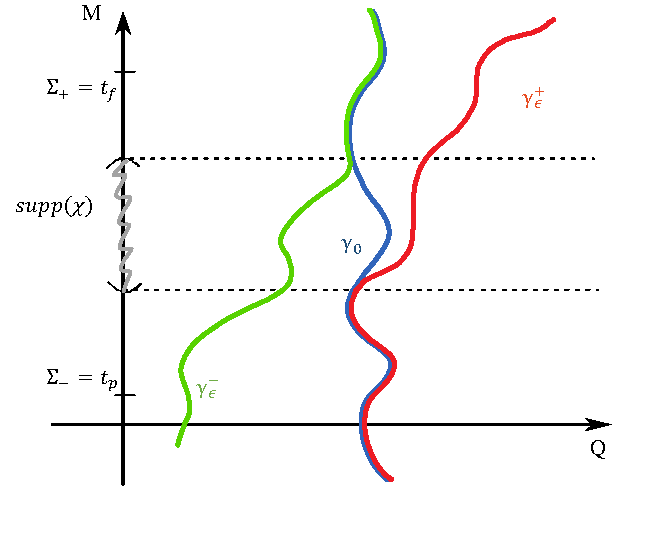
\includegraphics[width=0.5\textwidth]{./Pictures/AdvRetSol}}
  			%\includegraphics[keepaspectratio=true,scale=0.6]{slike/visina8}}
			\captionof{figure}{Picture of the perturbed solution in case of a finite dimensional system.}\label{GraphicAdvRetSol}%      only if needed  
			
			\end{minipage}
		
		Once seen as the perturbation $\epsilon \chi$ disturbs the solution $\gamma_0 \in \Sol$, it is possible to compute the effect of a perturbing density $\chi$ on the values of the functional $F_\omega$ associated to as second Lagrangian density $\omega$ as shown in equation \ref{EffectOperator}.
		By a Taylor expansion arrested to the first order we can say that:
		\begin{displaymath}
			F_\omega \left( \gamma_\epsilon^{\, \pm} \right) [f]= \int f(t) 
			\omega( t, \gamma_0^{\, i} + \epsilon \eta^i_\pm , \dot{\gamma}_0^{\, i} + \epsilon \dot{\eta}_\pm^i ) dt =
			F_\omega (\gamma_0) [f] + \epsilon \int f(t) \left[ 
			\left. \frac{\partial\omega}{\partial q^i}\right\vert_{\gamma_0} \eta^i_\pm +
			\left. \frac{\partial\omega}{\partial \dot{q}^i}\right\vert_{\gamma_0} \dot{\eta}^i_\pm 
			 \right] dt
		\end{displaymath}
		for any test function $f$.\\
		Substituting this result in the definition of effect operator:
		\begin{displaymath}
			\EffectOp_\chi^{\, \pm} F_\omega ( \gamma_0) [f] = \int f(t) \left[ 
			\left. \frac{\partial\omega}{\partial q^i}\right\vert_{\gamma_0} \eta^i_\pm +
			\left. \frac{\partial\omega}{\partial \dot{q}^i}\right\vert_{\gamma_0} \dot{\eta}^i_\pm 
			 \right] dt
		\end{displaymath}
		we get an explicit expression for the Peirels brackets:
		\begin{align}\label{EspressionePeierlsCampiCurve}
			\left\lbrace \chi , \omega \right\rbrace \left( \gamma_0 \right) [f] &=
			\int f(t) \left[ 
			\left.\left( \frac{\partial\omega}{\partial q^i}\right)\right\vert_{\gamma_0} \left( \eta_- - \eta_+\right)^i +
			\left.\left( \frac{\partial\omega}{\partial \dot{q}^i}\right)\right\vert_{\gamma_0} \left( \dot{\eta}_- - \dot{\eta}_+\right)^i 
			 \right] dt = \nonumber\\
			 &= \int f(t) 
			 \left[  
				\left.\left( \frac{\partial\omega}{\partial q^i}\right)\right\vert_{\gamma_0} +
				\left.\left( \frac{\partial\omega}{\partial \dot{q}^i}\right)\right\vert_{\gamma_0} \partial_t
			\right]
			\left[
				\left( \GreenAdv - \GreenRet \right)\left( - Q_\chi \gamma_0 \right)
			\right]^i				dt
		\end{align}
			
		
	 
	% Debug	
	%	\bibliography{bibliography}
	% \bibliographystyle{plain}	 	
	 	
\end{document}